\documentclass{beamer}

\usepackage{subfiles}
\usepackage{framed}
\usepackage{amsmath}
\usepackage{amssymb}


\begin{document}

%=================================================%
\begin{frame}
	\Huge
Introduction to ggvis

\begin{figure}
\centering
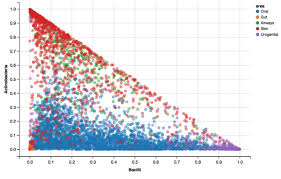
\includegraphics[width=0.8\linewidth]{ggvis1}
\end{figure}

\end{frame}
%=================================================%
% SPONSORS
% - Revolution Analytics
% - CPL
% - DIT 
%=================================================%
% PHASE 1 
%=================================================%
%=================================================%
\begin{frame}
\frametitle{Introduction to ggvis}
\LARGE
\textbf{Overview}
\begin{itemize}
%\item Recap of the basics of ggplot2
\item Getting started with ggvis
\item The magrittr \texttt{R} package and the $\%>\% $ operator
\item Common plot functions and managing aesthetics
\item Layers
\item Interactivity 
\end{itemize}
\end{frame}
%=================================================%
\begin{frame}
\frametitle{Resources}
\LARGE

\begin{itemize}
\item \texttt{R} (version 3.2)
\item RStudio
\item ggvis (version 0.4.1)
\item Version Particularly Important
\item Dataset : nycflights13 (R package)
\end{itemize}

\end{frame}
%================================================== %
\begin{frame}
	\begin{figure}
\centering
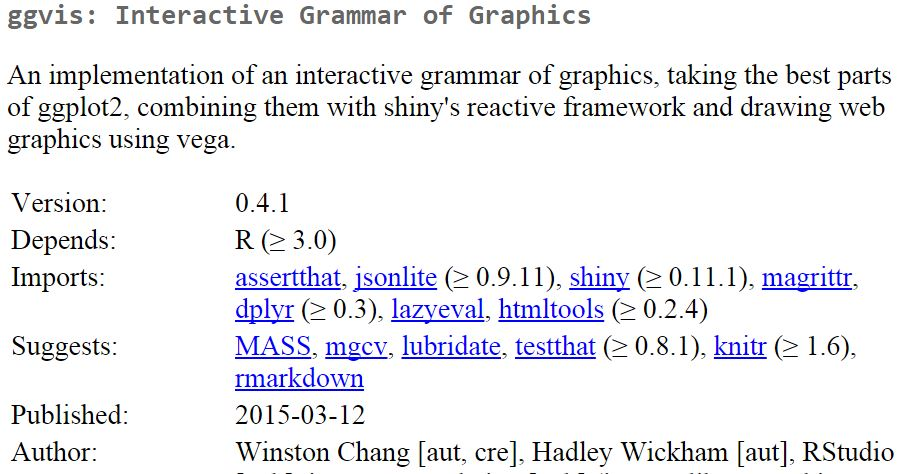
\includegraphics[width=1.05\linewidth]{images/CRAN-ggvis}

\end{figure}

\end{frame}
%=================================================%
\begin{frame}
	\frametitle{Using ggvis - a word of warning!}
	\begin{figure}
		\centering
		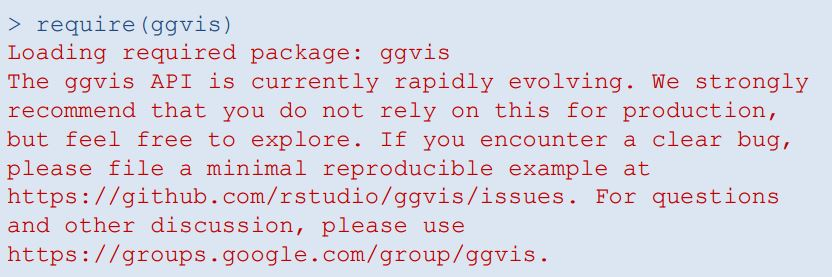
\includegraphics[width=1.05\linewidth]{ggviswarning}
		\caption{}
		\label{fig:ggviswarning}
	\end{figure}
	
\end{frame}
%================================================= %
\begin{frame}
	\begin{figure}
\centering
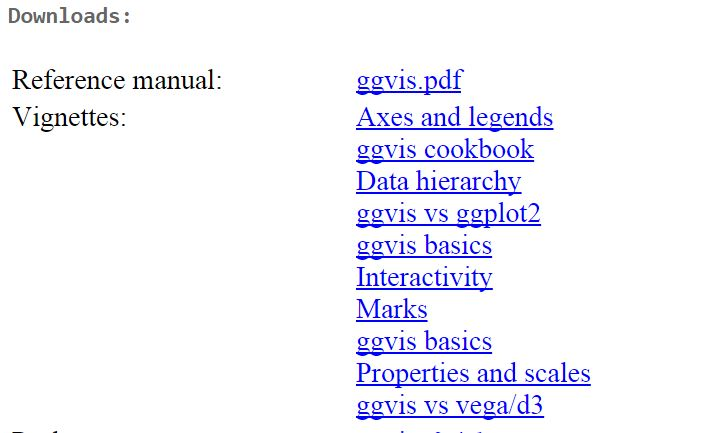
\includegraphics[width=1.05\linewidth]{images/CRAN-ggvis-vignettes}

\end{figure}

\end{frame}

%=================================================%
\begin{frame}[fragile]
\frametitle{The Data}
\begin{itemize}
\item All examples will be using tubeData
\item London Tube performance Data from the TFL
website
\item The original data can be found on

\end{itemize}
\begin{verbatim}
http://data.london.gov.uk/dataset/tube-networkperformance-data-transport-committee-report

\end{verbatim}
\end{frame}
%=================================================%
%\subfile{ggvis1-basic.tex}  

\subfile{ggplot2revision.tex}

%=================================================%
%=================================================%
%PHASE 2
%=================================================%
%=================================================%
\begin{frame}
	\huge
	Introduction to ggvis
	
	\begin{itemize}
		\item Installing ggvis
		\item Our first plot
		\item Useful things to know (magrittr)
	\end{itemize}
	
\end{frame}
\subfile{ggvis1-firstplot.tex}

\subfile{ggvis1-vega.tex}

\subfile{magrittr.tex} % NOT READY

\subfile{ggvis1-basic-examples.tex}

%=================================================%
\begin{frame}[fragile]
\begin{framed}
\begin{verbatim}
tubeData %>%
    ggvis(x = ~Month, y = ~Excess) %>%
        layer_points()
\end{verbatim}
\end{framed}
\begin{figure}
\centering
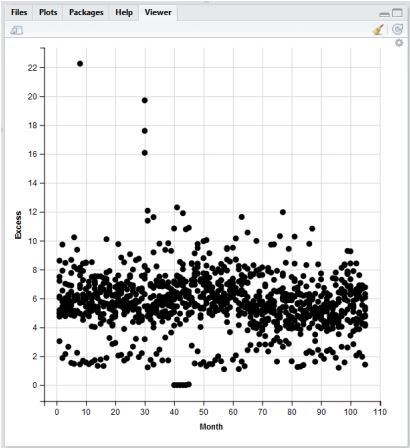
\includegraphics[width=0.5\linewidth]{got-ggvisplot1}
\end{figure}

\end{frame}
%=================================================%
%=================================================%
%PHASE 3
%=================================================%
%=================================================%

\subfile{ggvis2-aesthetics.tex}
\subfile{ggvis2-commonplotfunctions.tex}
\subfile{ggvis3-layers.tex}



%=================================================%
%=================================================%
% Phase 4
%=================================================%
%=================================================%

\subfile{ggvis2-interactivity.tex}
\subfile{ggvis2-interactivity-more.tex}
\subfile{ggvis4-MultipleLayers.tex}
% \subfile{ggvis5-moredetails.tex}

\end{document}
